\section{Superconductivity - The Bogoliubov-de-Gennes Formalism}
Last time, we looked at the historic approach the BCS theory. Today we basically do the same thing, but using a modern formalism. It is faster, more elegant, and lets us calculate things with less effort. This is not too surprising - the beginning of a theory is always the most difficult. Eventually, others come up with more efficient and useful formulations/extensions. In the formalism we discuss today, we can consider superconductivity at finite temperature (vs. last lecture whose results were only applicable at $T = 0$).

\subsection{The Bogoliubov-de-Gennes Hamiltonian}
The BDG approach seeks to solve the BCS pairing Hamiltonian:
\begin{equation}\label{eq-BCSpairingH}
    H = \sum_{\v{k}, \sigma} \xi_{\v{k}}c^\dag_{\sigma\v{k}}c_{\sigma\v{k}} + \sum_{\v{k}\v{l}}V_{\v{k}\v{l}}c^\dag_{\v{k}\uparrow}c^\dag_{-\v{k}\downarrow}c_{-\v{l}\downarrow}c_{\v{l}\uparrow}
\end{equation}
via a mean-field decoupling. We take the interaction term and write it in the mean-field approximation:
\begin{equation}
    c^\dag_{\v{k}\uparrow}c^\dag_{-\v{k}\downarrow}c_{-\v{l}\downarrow}c_{\v{l}\uparrow} \to c^\dag_{\v{k}\uparrow}c^\dag_{-\v{k}\downarrow}\avg{c_{-\v{l}\downarrow}c_{\v{l}\uparrow}} + \avg{c^\dag_{\v{k}\uparrow}c^\dag_{-\v{k}\downarrow}} c_{-\v{l}\downarrow}c_{\v{l}\uparrow} - \avg{\ldots}(\ldots).
\end{equation}
Sometimes this is called ``Hartree-Fock in the pairing channel''. Normally we pair $c^\dag$s with $c$s, but in the superconductiviy problem we pair $c^\dag$s together and $c$s together. If we recall the form of the BCS ground state, there is a $c^\dag c^\dag$ arising so we expect nonzero expectation value even when taking expectation values of operators of the same type. In this approximation, Eq. \eqref{eq-BCSpairingH} can be approximated as:
\begin{equation}
    H_{BdG} = \sum_{\v{k}\sigma}\xi_{\v{k}}c^\dag_{\v{k}\sigma}c_{\v{k}\sigma} + \sum_{\v{k}}\left(\Delta_{\v{k}}c^\dag_{\v{k}\uparrow}c^\dag_{-\v{k}\downarrow} + \text{h.c.}\right) + \sum_{\v{k}}\Delta_{\v{k}}\avg{c^\dag_{\v{k}\uparrow}c^\dag_{-\v{k}\downarrow}}
\end{equation}
where:
\begin{equation}
    \Delta_{\v{k}} = \sum_{\v{l}}V_{\v{k}\v{l}}\avg{c_{-\v{l}\downarrow}c_{\v{l}\uparrow}}
\end{equation}
is the ``pairing field''. We can now diagonalize this using a canonical/unitary transformation.

Customarily, one defines a Nambu spinor:
\begin{equation}
    \psi_\v{k} = \m{c_{\v{k}\uparrow} \\ c^\dag_{-\v{k}\downarrow}}
\end{equation}
Which allows one to write $H_{BdG}$ in the compact form:
\begin{equation}\label{eq-HBdGcompact}
    \begin{split}
        H_{BdG} &= \sum_{\v{k}} \psi_{\v{k}}^\dag \m{\xi_{\v{k}} & \Delta_{\v{k}} \\ \Delta_{\v{k}}^* & -\xi_{\v{k}}}\psi_{\v{k}} + E_0
        \\ \text{where }  E_0 &= \sum_{\v{k}}\xi_{\v{k}} - \sum_{\v{k}}\Delta_{\v{k}}\avg{c^\dag_{\v{k}\uparrow}c^\dag_{-\v{k}\downarrow}}
    \end{split}
\end{equation}
where the $\sum_{\v{k}}\xi_{\v{k}}$ comes from the anticommutation relations which generates a constant. The 2x2 matrix $h_\v{k} = \m{\xi_{\v{k}} & \Delta_{\v{k}} \\ \Delta_{\v{k}}^* & -\xi_{\v{k}}}$ has eigenvalues $\pm E_\v{k}$ with:
\begin{equation}
    E_{\v{k}} = \sqrt{\xi_{\v{k}}^2 + \abs{\Delta_{\v{k}}}^2}
\end{equation}
In the diagonal basis, we find the BdG Hamiltonian Eq. \eqref{eq-HBdGcompact} becomes:
\begin{equation}\label{eq-BdGdiagonal}
    H_{BdG} = \sum_{\v{k}}E_{\v{k}}\left(\gamma^\dag_{\v{k}_1}\gamma_{\v{k}_1} - \gamma^\dag_{\v{k}_2}\gamma_{\v{k}_2}\right) + E_0
\end{equation}
Here, $\gamma_{\v{k}\alpha}$ are the BdG quasiparticle operators (still fermions!) related to $c_{\v{k}\sigma}$ via a unitary transformation (that diagonalizes the Hamiltonian):
\begin{align*}
    \m{\gamma_{\v{k}1} \\ \gamma_{\v{k}2}} = U_\v{k}\m{c_{\v{k}\uparrow} \\ c^\dag_{-\v{k}\downarrow}}.
\end{align*}
An interesting connection with our previous discussion of BCS theory. If we look at $U_\v{k}$:
\begin{align*}
    U_{\v{k}} = \m{u_{\v{k}} & v_\v{k}^* \\ v_{\v{k}} & -u_{\v{k}}^*}
\end{align*}
where $u_{\v{k}}, v_{\v{k}}$ were the coefficients appearing in the BCS ground state wavefunction we obtained last class.

\subsection{Bogoliubov-de-Gennes Ground State and Excitations}
By definition, $E_{\v{k}}$ is positive. So it is very easy to create a ground state. If there were any $\gamma_{\v{k}1}$ particles in the ground state, this would cost energy (note the plus sign); conversely, $\gamma_{\v{k}2}$ particles take away energy (note the minus sign). So, the ground state would have no $\gamma_{\v{k}1}$ particles and all $\gamma_{\v{k}2}$ particles.

We therefore write:
\begin{equation}
    \ket{\Psi_G} = \prod_{\v{k}}\gamma^\dag_{\v{k}2}\ket{0}
\end{equation}
and it can be shown that this is equivalent to the BCS ground state. 

The new contribution of this formalism is the ability to discuss excitations above the ground state. Excitations/increasing energy would involve either adding a $\gamma_{\v{k}1}$ particle or removing a $\gamma_{\v{k}2}$ particle, each of which costs energy. This implies an interpretation of $E_{\v{k}}$ as the excitation spectrum of the superconductor. This is nice because we are now able to discuss thermodynamic quantities and transport properties (the BCS approach only gives us the ground state). One last note - whenever we have a property such that $\min_{\v{k}}\abs{\Delta_{\v{k}}} > 0$, the excitation spectrum is gapped - namely it costs finite energy to produce the excitation. And this can be see from the form $E_\v{k} = \sqrt{\xi_\v{k}^2 + \abs{\Delta_{\v{k}}}^2}$ - $\xi_{\v{k}} = \e_{\v{k}} - \mu$ can vanish at the Fermi surface, but if $\min_{\v{k}}\abs{\Delta_{\v{k}}} > 0$ then $E_{\v{k}} > 0$ for all $\v{k}$. Note that this property is true for most, but not all superconductors. In fact, superconductors which have gapped excitations are considered to be conventional superconductors. However, there are examples (e.g. high $T_c$ cuprates) where this does not hold. As a result, $\Delta_{\v{k}}$ is often called the superconducting gap function. 

\subsection{Temperature Dependence of Superconductors}
We defined $\Delta_{\v{k}}(T)$, but we still must calculate it. This will allow us to obtain the critical temperature (and later, specific heat) of the superconductor. It can be determined by minimizing the system free energy - which we recall to be $F = -\frac{1}{\beta}\ln Z$ from statistical mechanics, with $Z$ the partition function. The general expression for $Z$ is:
\begin{equation}
    \begin{split}
        Z &= \sum_{\set{n}} e^{-\beta E\set{n}}
        \\ \text{where } E\set{n} &= \sum_{\v{k}}E_{\v{k}}(n_{\v{k}_1} - n_{\v{k}_2}) + E_0
    \end{split}
\end{equation}
(which can be read off directly from the Hamiltonian) and $n_{\v{k}\alpha} = 0, 1$. From this, we are able to calcualte the partition function:
\begin{equation}
    \begin{split}
        Z &= \sum_{n_{\v{k}1}, n_{\v{k}2}} e^{-\beta\sum_{\v{k}}E_{\v{k}}n_{\v{k}1}}e^{\beta\sum_{\v{k}}E_{\v{k}}n_{\v{k}2}}e^{-\beta E_0}
        \\ &= e^{-\beta E_0}\prod_{\v{k}}\left(1 + e^{-\beta E_{\v{k}}}\right)\left(1 + e^{\beta E_{\v{k}}}\right)
        \\ &= e^{-\beta E_0}\prod_\v{k}\left(e^{\frac{1}{2}\beta E_{\v{k}}} + e^{-\frac{1}{2}\beta E_{\v{k}}}\right)^2
        \\ &= e^{-\beta E_0}\prod_{\v{k}}(2\cosh \frac{1}{2}\beta E_{\v{k}})^2
    \end{split}
\end{equation}
Now, we take a logarithm (and divide by $-\beta$) to get the free energy:
\begin{equation}
    F = E_0 - \frac{1}{\beta}\sum_{\v{k}}2\ln(2\cosh\frac{1}{2}\beta E_\v{k})
\end{equation}
Where we recall that $E_{\v{k}} = \sqrt{\xi_{\v{k}}^2 + \Delta_\v{k}^2}$ and $E_0 = \sum_{\v{k}}\xi_{\v{k}} - \sum_{\v{k}}\Delta_{\v{k}}\avg{c^\dag_{\v{k}\uparrow}c^\dag_{-\v{k}\downarrow}}$. We again adopt the Cooper ansatz for $V_{\v{k}\v{l}}$, which implies:
\begin{align*}
    \Delta_{\v{k}} = \begin{cases}
        \Delta = -V\sum_{\v{l}}'\avg{c_{-\v{l}\downarrow}c_{\v{l}\uparrow}} & \abs{\xi_{\v{k}}} < \hbar \omega_c
        \\ 0 & \text{otherwise}
    \end{cases}
\end{align*}
and this has the convenient implication:
\begin{equation}
    E_0 = \sum_{\v{k}}\xi_{\v{k}} + \frac{1}{V}\Delta^2
\end{equation}
so now we are able to minimize $F$ with respect to $\Delta$:
\begin{equation}
    0 = \dpd{F}{\Delta} = \frac{2}{V}\Delta - 2\sum_{\v{k}}\dpd{E_\v{k}}{\Delta}\tanh\frac{1}{2}\beta E_{\v{k}}, \quad \dpd{E_{\v{k}}}{\Delta} = \frac{\Delta}{E_{\v{k}}}
\end{equation}
Finally, we get what is known as the BCS gap equation at non-zero $T$:
\begin{equation}\label{eq-BCSgap}
    \frac{\Delta}{V} = \frac{1}{2}\sum_{\v{k}}'\frac{\Delta}{E_{\v{k}}}\tanh\frac{1}{2}\beta E_{\v{k}}
\end{equation}
which self-consistently determines $\Delta$ as a function of temperature. Let's analyze this - we can learn something interesting from it.

At $T = 0$ $\beta = \infty$ and so $\tanh \frac{1}{2}\beta E_\v{k} = 1$. So we then obtain:
\begin{align*}
    \frac{\Delta}{V} = \frac{1}{2}\sum_{\v{k}}'\frac{\Delta}{E_{\v{k}}}
\end{align*} 
we already solved this on Monday to obtain:
\begin{equation}\label{eq-Delta0}
    \Delta \approx 2\hbar \omega_c e^{-1/N(0)V}
\end{equation}
so we reproduce the zero-temperature result. At a generic nonzero temperature, Eq. \eqref{eq-BCSgap} is a transcendental equation that must be solved via numerical iteration (i.e. start with some value for $\Delta_0$, compute the new value by evaluating the sum to get $\Delta_1$, and iterate until convergence). One obtains:

\begin{figure}[htbp!]
    \centering
    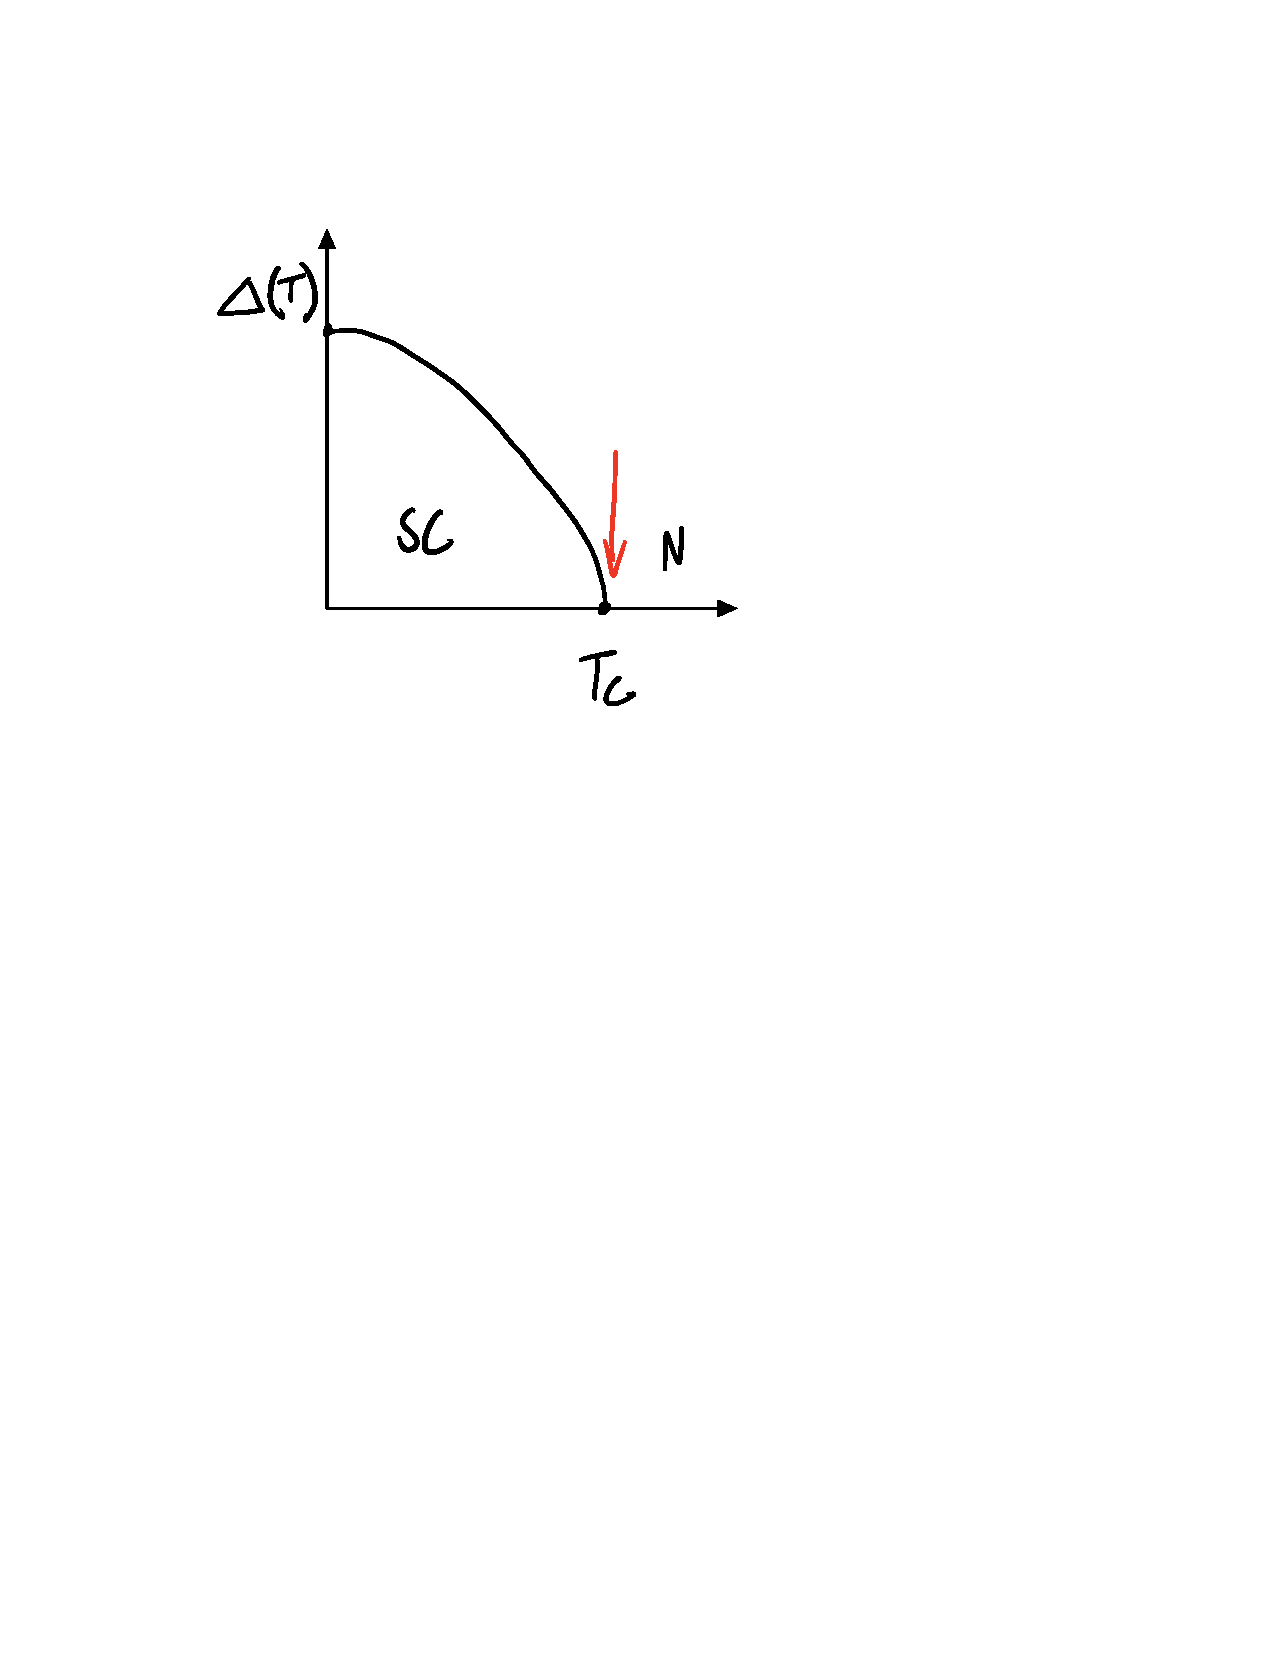
\includegraphics[scale=0.7]{Images/fig-scdelta.pdf}
    \caption{Plot of the superconducting gap function $\Delta(T)$ as a function of temperature. $\Delta$ acts as an order parameter, where it is positive in the superconducting phase and zero outside of it. $\Delta$ goes to 0 at the critical temperature $T_c$, where the phase transition (denoted by the red arrow) occurs.}
    \label{fig-scdelta}
\end{figure}

and we find that near the phase transition:
\begin{equation}
    \frac{\Delta(T)}{\Delta(0)} \approx 1.74\left(1 - \frac{T}{T_c}\right)^{1/2}
\end{equation}
with $T_c$ the critical temperature. Note mean-field theory provides us the critical exponent of $1/2$. However it is of course worth noting that these critical exponents are universal information (determined, e.g. by the symmetries of the Hamiltonian and dimensionality), and they are often of interest to study and determine in CM research. $\Delta$ acts as an order parameter for this phase transition, where $\Delta(T) = 0$ for $T \geq T_c$ and $\Delta(T) > 0$ for $T < T_c$.

\subsection{Determining the Critical Temperature}
As $\Delta(T) \to 0$, we replace in Eq. \eqref{eq-BCSgap} $E_k \to \abs{\xi_{\v{k}}}$ and solve:
\begin{equation}
    \begin{split}
        \frac{1}{V} &= \frac{1}{2}\sum_{\v{k}}' \frac{1}{\xi_{\v{k}}}\tanh \frac{1}{2}\beta \xi_{\v{k}}
        \\ &= N(0)\int_0^{\hbar \omega_c}d\xi \frac{1}{\xi} \tanh \frac{1}{2}\beta \xi
        \\ &= N(0)\ln(\frac{2\gamma}{\pi} \beta \hbar \omega_c)
    \end{split}
\end{equation}
where $\gamma$ is the Euler constant, and $\frac{2\gamma}{\pi} \approx 1.13$. The critical temperature is then obtained as:
\begin{equation}
    k_B T_C = \frac{1}{\beta_C} = 1.13\hbar \omega_c e^{-1/N(0)V}
\end{equation}

What is usually done is to find the BCS universal ratio (dividing by \eqref{eq-Delta0}):
\begin{equation}
    \frac{\Delta(0)}{k_B T_c} = \frac{2}{1.13} = 1.76
\end{equation}
Both $\Delta(0)$ and $T_c$ are measurable. One finds experimental values of $\Delta(0)/k_B T_c$ to range between 1.5-2.3 in most conventional superconductors, in agreement with the theoretical prediction. There are of course unconventional superconductors like high-$T_c$ cuprates where the value can differ quite significantly (3-4). 

\subsection{Specific Heat of Superconductors}
The specific heat of electrons in a superconductor is most easily obtained from entropy, using the thermodynamic identity:
\begin{equation}
    C_{ls} = T\dod{S_{ls}}{T} = -\beta\dpd{S_{ls}}{\beta}
\end{equation}
where $S_{ls}$ denotes the entropy of the Fermion gas in Eq. \eqref{eq-BdGdiagonal}, which is:
\begin{equation}
    S_{ls} = -2k_B\sum_{\v{k}}\left[(1-n_{\v{k}})\ln(1 - n_{\v{k}}) + n_{\v{k}}\ln n_{\v{k}}\right]
\end{equation}
Which we now evaluate:
\begin{equation}
    \begin{split}
        C_{ls} &= 2\beta k_B \sum_{\v{k}}\dpd{n_{\v{k}}}{\beta}\ln\frac{n_{\v{k}}}{1 - n_{\v{k}}} 
        \\ &= -2\beta^2 k_B \sum_{\v{k}}E_{\v{k}}\dpd{n_{\v{k}}}{\beta}
        \\ &= -2\beta^2k_B\sum_{\v{k}}E_{\v{k}} \dod{n_{\v{k}}}{(\beta E_{\v{k}})}(E_{\v{k}} + \beta \dod{E_{\v{k}}}{\beta})
        \\ &= 2\beta k_B \sum_{\v{k}}\left(-\dpd{n_{\v{k}}}{E_{\v{k}}}\right)\left(E_{\v{k}}^2 + \frac{1}{2}\beta \dod{\Delta^2}{\beta}\right)
    \end{split}
\end{equation}
Sketching this:

\begin{figure}[htbp]
    \centering
    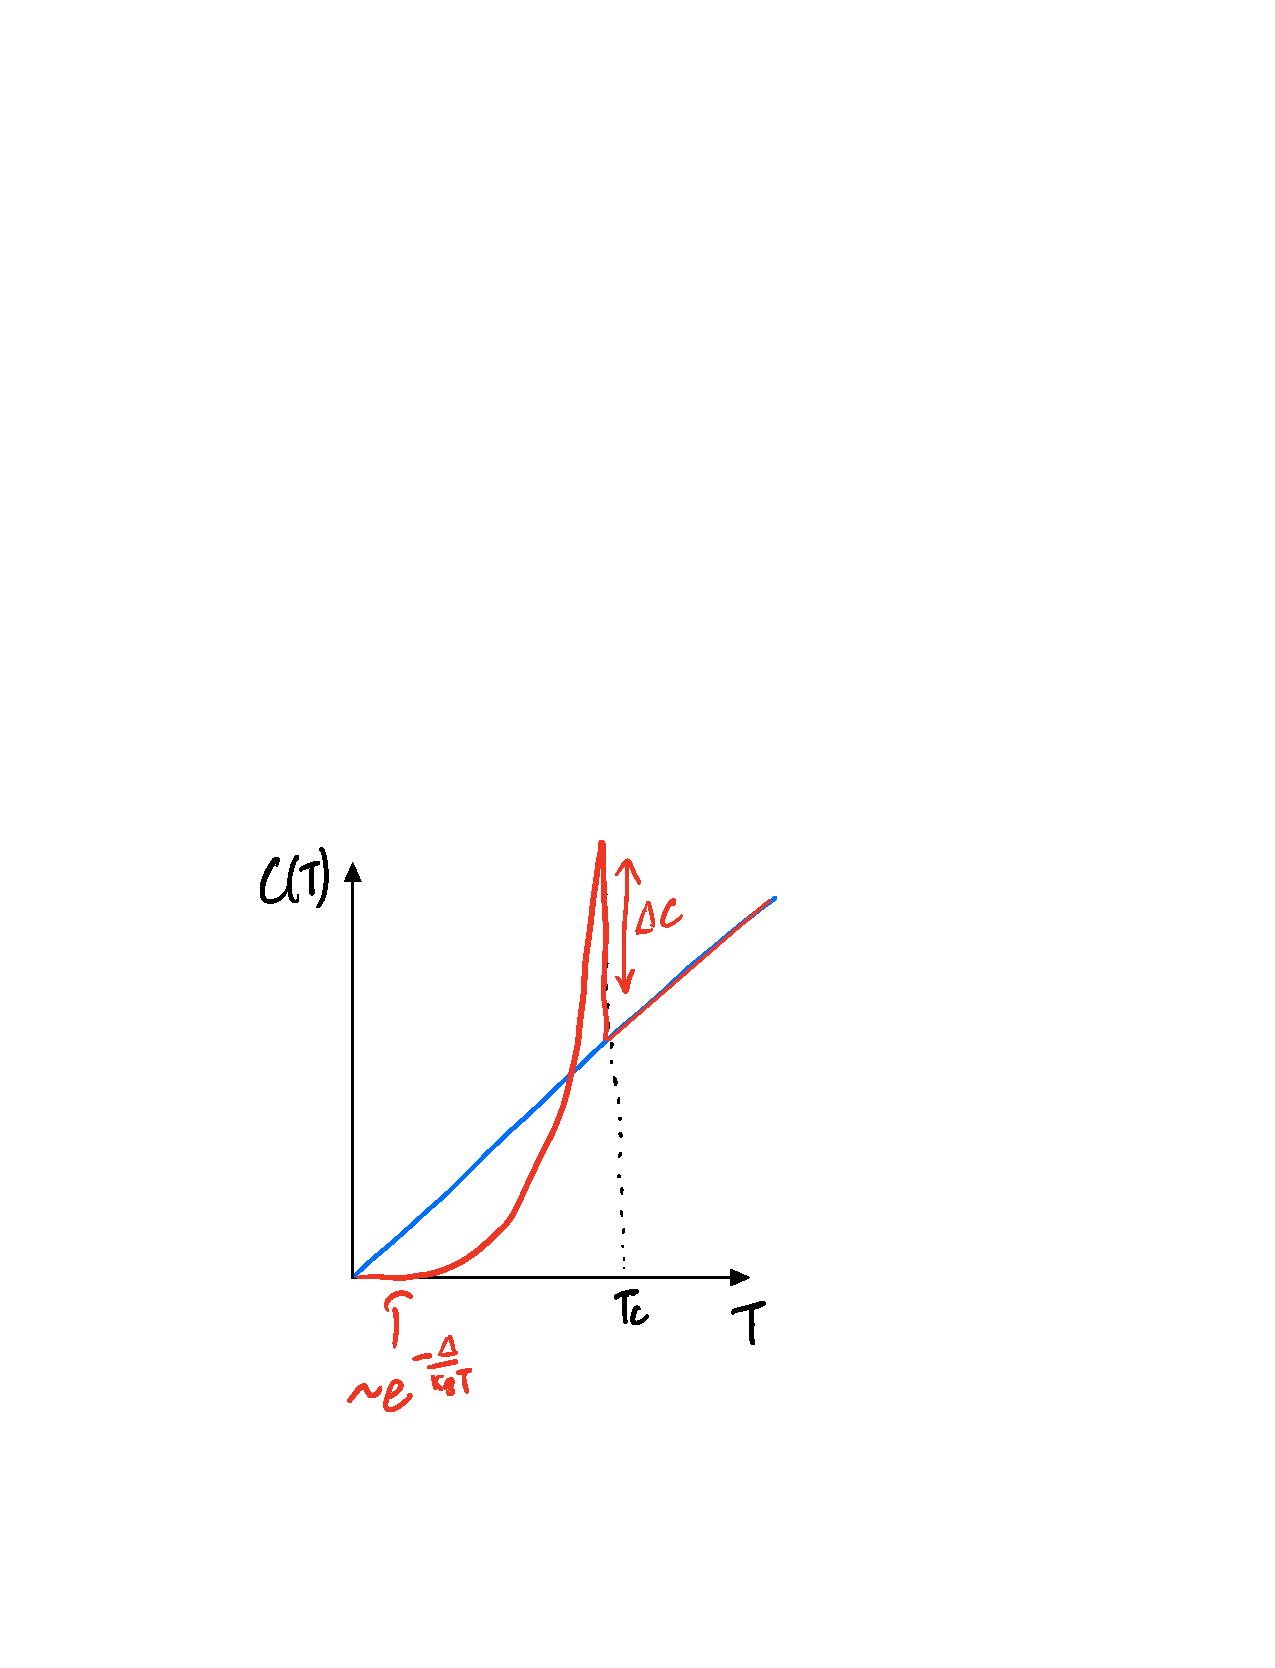
\includegraphics[scale=0.7]{Images/fig-scheatcapacity.pdf}
    \caption{Plot of the heat capacity of a superconductor $C_{ls}$ as a function of temperature (red), compared with a normal metal $C_{ln}$ (blue, linear in $T$). There is exponential activation at low $T$ (like an insulator), and then the heat capacity steeply rises, before dropping down at $T_c$ and increasing linearly in $T$ thereafter (where we have now left the superconducting phase, and the material acts like a regular metal).}
    \label{fig-scheatcapacity}
\end{figure}

Note the exponential activation at low temperatures. Also, note the superconductor phase transition at $T_c$ is marked by a jump $\Delta C$ in $C$, which is characterized by the universal ratio:
\begin{equation}
    \frac{\Delta C}{C_{ln}(T_c)} \approx 1.43
\end{equation}
which is in agreement with experimental measurements.

If we had more time, we could calculate many other things from this theory - the zero-resistivity, the Meissner effect (expelling of magnetic fields, which exponentially decay in the superconductor, with characteristic London scale $\lambda$).

\begin{figure}[htbp]
    \centering
    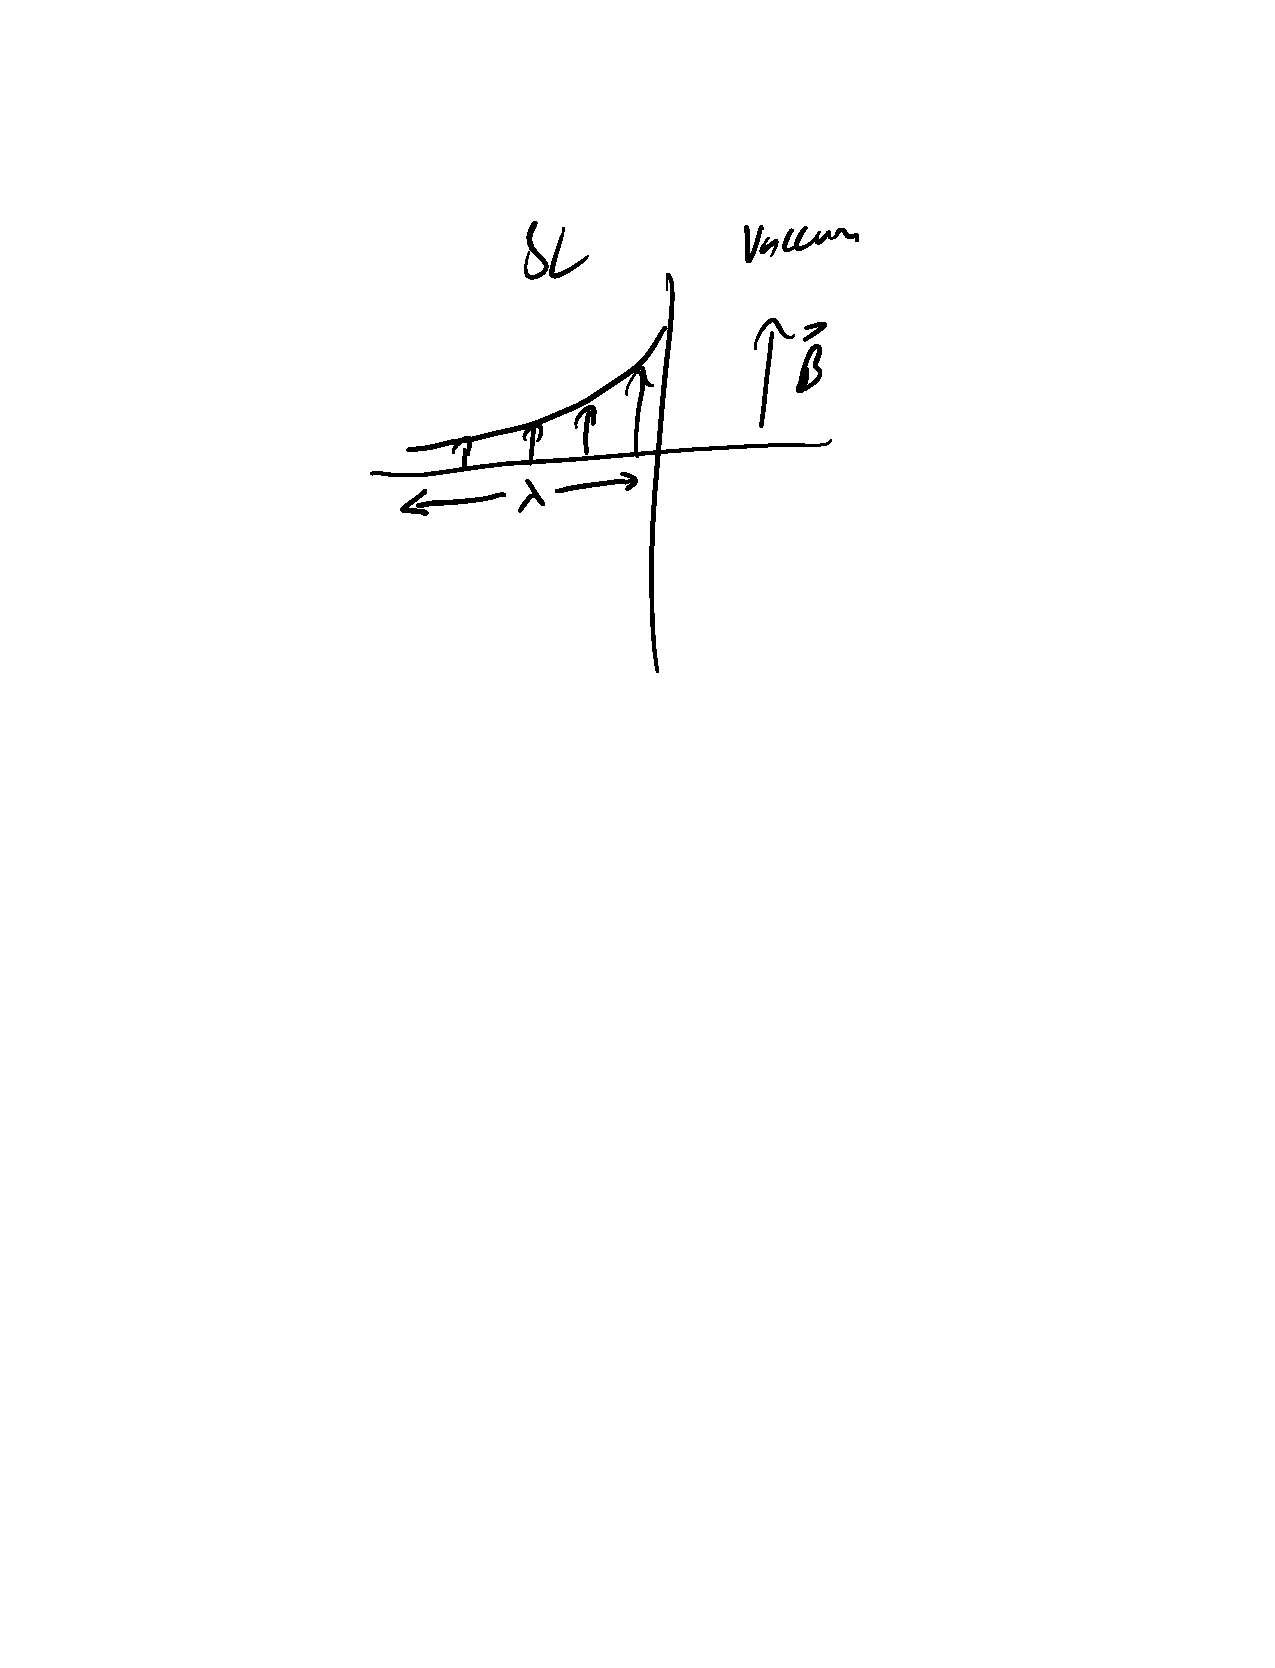
\includegraphics[scale=0.7]{Images/fig-meissener.pdf}
    \caption{Cartoon of how the magnetic fields in a superconductor drops off exponentially inside of it, with characteristic London scale $\lambda$.}
    \label{fig-meissener}
\end{figure}